\documentclass[11pt,a4paper]{article}
\usepackage{../shared/luxcover}
\usepackage[utf8]{inputenc}
\usepackage[T1]{fontenc}
\usepackage{amsmath,amssymb,amsfonts}
\usepackage{amsthm}
\usepackage{graphicx}
\usepackage{hyperref}
\usepackage{booktabs}
\usepackage{enumitem}
\usepackage{xcolor}
\usepackage{siunitx}
\usepackage{listings}
\usepackage{tikz}
\usetikzlibrary{arrows.meta,positioning,fit,backgrounds}

\hypersetup{colorlinks=true,linkcolor=black,citecolor=blue,urlcolor=blue}

\lstset{
  basicstyle=\ttfamily\scriptsize,
  breaklines=true,
  frame=single,
  showstringspaces=false,
}

\newcommand{\msg}[1]{\textsf{#1}}
\newcommand{\code}[1]{\texttt{#1}}
\newtheorem{theorem}{Theorem}
\newtheorem{lemma}{Lemma}
\newtheorem{definition}{Definition}
\newtheorem{claim}{Claim}
\newtheorem{assumption}{Assumption}

\title{A Unified Post-Quantum Transport for Lux:\\
       QUIC-over-ZAP, One Port per Validator}
\author{Lux Industries, Inc. \\
        \texttt{research@lux.network}}
\date{2026-06-30 \quad (LP-202, Draft --- Design \& Specification)}

\begin{document}
\luxcoverpage

\begin{abstract}
We specify a single post-quantum transport that collapses a Lux
validator's three network endpoints --- \code{9630} HTTP-RPC,
\code{9631} classical staking-P2P, and \code{9632} ZAP-native RPC ---
onto \emph{one} UDP port carrying QUIC over ZAP. Three stream classes
(RPC, consensus-P2P, ZAP-native services) are multiplexed on one
connection, eliminating cross-class head-of-line blocking. Every
connection is end-to-end post-quantum: confidentiality and key
agreement come from the IANA hybrid group \code{X25519MLKEM768}
(0x11EC) in the QUIC TLS~1.3 handshake, and peer authentication is a
hybrid \emph{classical\,$\wedge$\,ML-DSA-65} validator identity that
preserves the existing 20-byte hash-of-hash \code{NodeID} while binding
a FIPS-204 signing key channel-bound to the QUIC session.

This is a \emph{transport} change only. The Lux consensus message set
(the P2P message set Lux inherited from its Avalanche fork) and the BFT
decision logic are unchanged byte-for-byte; consensus messages ride QUIC
streams instead of a shared TCP byte stream. The
proven classical TCP staking path (\code{9631}) remains the negotiated
fallback: validators upgrade \emph{to} QUIC-PQ and never retire the
classical path until a devnet A/B test proves \emph{byte-identical
finality}. We give the wire format, the hybrid handshake and its
channel binding, the message-to-stream map, capability negotiation for
mixed fleets, the per-network DNS scheme
(\code{$\langle$NN$\rangle$.lux.network}), the A/B acceptance
methodology, and an argument that the transport change does not alter
$f<n/3$ safety or liveness. The design reuses \code{luxfi/zap}'s
QUIC + \code{X25519MLKEM768} transport, its \code{SPEC-ZAP-PQ-v1}
(``Z-Wing'') hybrid handshake, luxd's already-present ML-DSA-65
\code{NodeID} scheme, and the \code{node2} leaderless BLS vote-mesh ---
nothing is forked. We are explicit throughout about what is
\emph{proven and live} versus what is \emph{specified here and not yet
built}.
\end{abstract}

\tableofcontents
\newpage

%======================================================================
\section{Introduction}\label{sec:intro}

A Lux validator today speaks three network dialects on three sockets:

\begin{itemize}[nosep]
  \item \code{:9630} --- HTTP/JSON-RPC for the \code{/ext/*} client API
        (\code{DefaultHTTPPort}).
  \item \code{:9631} --- a single long-lived TCP stream per peer carrying
        \emph{all} Lux P2P and consensus traffic
        (\code{DefaultStakingPort}), authenticated by a TLS~1.3 staking
        certificate.
  \item \code{:9632} --- an opt-in ZAP-native RPC listener
        (\code{ZAP\_RPC\_LISTEN}) that re-serves the same \code{/ext/*}
        handler chain over the ZAP wire codec.
\end{itemize}

Three ports means three firewall holes, three TLS stances, three
DoS surfaces, three sets of health checks, and --- most importantly ---
\emph{no shared post-quantum posture}. The staking TCP stream also
suffers transport head-of-line (HOL) blocking: a slow bootstrap
\msg{GetAncestors} transfer and a latency-critical \msg{PushQuery} share
one ordered byte stream, so a stalled fetch delays a consensus vote.

This document specifies the endpoint of a different design: \textbf{one
UDP port per validator}, QUIC over ZAP, end-to-end post-quantum, with
RPC, consensus-P2P, and ZAP-native services multiplexed as independent
QUIC streams. The change is deliberately confined to the transport. We
do not touch the consensus engine, the proposer VM, the message
definitions, or the BFT decision rule. Consensus messages are the same
bytes; they simply travel on a QUIC stream rather than a TCP segment.

\subsection{Design tenets}

\begin{enumerate}[nosep]
  \item \textbf{Decomplect transport from consensus.} The BFT logic
        already sits behind a transport-agnostic seam (the \code{Upgrader}
        and \code{EndpointDialer} interfaces, \S\ref{sec:seam}). A new
        transport is a new implementation of that seam, not a change to
        the seam's consumers.
  \item \textbf{Extend, do not break.} TCP staking on
        \code{9631} stays as the proven baseline. QUIC-PQ is a
        \emph{capability} a validator negotiates \emph{up} to. Mixed
        fleets interoperate; there is no flag day.
  \item \textbf{Reuse, do not fork.} Every cryptographic and wire
        primitive already exists in tree: \code{luxfi/zap}'s QUIC
        transport with \code{X25519MLKEM768}
        (\S\ref{sec:proven-quic}); its \code{SPEC-ZAP-PQ-v1} hybrid
        handshake (\S\ref{sec:proven-zappq}); luxd's ML-DSA-65
        \code{NodeID} scheme and \code{PQHandshake}
        (\S\ref{sec:proven-pqid}); and \code{node2}'s leaderless BLS
        vote-mesh (\S\ref{sec:proven-node2}). This paper is mostly
        \emph{composition}.
  \item \textbf{Honesty about maturity.} \S\ref{sec:proven} enumerates
        what is proven and live. Everything else is labelled
        \emph{[design]}. The acceptance gate (\S\ref{sec:ab}) is the
        line a build must cross before the fallback is retired.
\end{enumerate}

\subsection{Contributions}

\begin{itemize}[nosep]
  \item A one-port wire model with a three-class stream demultiplexer and
        an analysis of the 0-RTT, connection-migration, and
        no-HOL-blocking properties (\S\ref{sec:wire}).
  \item A hybrid post-quantum handshake: \code{X25519MLKEM768} for the
        confidential channel plus a channel-bound ML-DSA-65 identity
        proof that preserves the 20-byte classical \code{NodeID} and
        upgrades it to a \emph{classical\,$\wedge$\,PQ} value
        (\S\ref{sec:handshake}). This closes a real gap: the shipped
        QUIC transport authenticates the \emph{channel} (TLS cert) but
        exchanges the ZAP \code{NodeID} as an \emph{unauthenticated}
        string (\S\ref{sec:gap}).
  \item A byte-preserving map of the full Lux/Simplex message set
        onto QUIC stream classes, reusing the \code{node2} vote-mesh
        semantics (\S\ref{sec:consensus}).
  \item A capability-negotiation scheme for mixed TCP/QUIC fleets
        (\S\ref{sec:fallback}), a per-network DNS scheme and a
        NAT/local-fiber validator join procedure (\S\ref{sec:dns}).
  \item A devnet A/B methodology that gates retirement of the fallback
        on byte-identical finality (\S\ref{sec:ab}), and a proof sketch
        that the transport swap preserves $f<n/3$ safety and liveness
        (\S\ref{sec:bft}).
\end{itemize}

%======================================================================
\section{Threat model and goals}\label{sec:threat}

\subsection{Adversary}

We assume a network adversary with the standard partial-synchrony
BFT powers, augmented with a store-now-decrypt-later quantum capability:

\begin{itemize}[nosep]
  \item \textbf{Network (Dolev--Yao).} Full control of the UDP/IP
        substrate: observe, drop, reorder, inject, replay, and delay
        packets; spoof source addresses; mount reflection/amplification
        and address-migration attacks against QUIC.
  \item \textbf{Byzantine participants.} Up to $f<n/3$ of validator
        stake is adversarial and may equivocate, withhold, or send
        arbitrary (but well-typed) messages. This is the \emph{message
        layer's} model and is unchanged by this document.
  \item \textbf{Harvest-then-decrypt quantum adversary.} Records all
        ciphertext now and runs a cryptographically-relevant quantum
        computer \emph{later}. Confidentiality of \emph{today's} traffic
        must survive \emph{tomorrow's} quantum computer; hence hybrid PQ
        key agreement is mandatory, not optional.
  \item \textbf{Future quantum forger.} May eventually break ECDLP
        (Shor), so long-lived \emph{authentication} must not rest on a
        classical assumption alone.
\end{itemize}

\subsection{Security goals}

\begin{enumerate}[nosep]
  \item[G1] \textbf{PQ confidentiality with forward secrecy.} Session
        keys are IND-CCA secure if \emph{either} X25519 \emph{or}
        ML-KEM-768 is unbroken; compromise of a validator's long-term
        signing key does not retroactively decrypt recorded sessions.
  \item[G2] \textbf{Hybrid peer authentication.} Impersonating a
        validator requires forging \emph{both} the classical staking
        credential \emph{and} an ML-DSA-65 signature. A quantum forger
        that breaks ECDLP alone cannot impersonate; a lattice break that
        does not also break the classical leg cannot either. (The
        ``X-Wing pattern'' applied to identity.)
  \item[G3] \textbf{\code{NodeID} continuity.} The value that keys the
        validator set --- the 20-byte hash-of-hash \code{NodeID} --- is
        preserved across the transport change so no re-registration or
        stake-map migration is forced.
  \item[G4] \textbf{Channel binding.} An authentication proof captured on
        one connection cannot be replayed onto another connection, chain,
        or epoch (defeats relay/MITM and cross-chain replay).
  \item[G5] \textbf{Transport-transparent BFT.} The consensus safety and
        liveness properties proven at the message layer hold unchanged
        under the new transport (\S\ref{sec:bft}).
  \item[G6] \textbf{Graceful coexistence.} A QUIC-PQ validator and a
        TCP-only validator reach the \emph{same finality}; the fleet is
        never partitioned by capability (\S\ref{sec:fallback}).
\end{enumerate}

\emph{Non-goals.} We do not redesign the BFT protocol, do not alter the
message schema, do not claim a NIST-certified \emph{threshold} scheme
(the identity keys here are single-signer ML-DSA-65 per validator), and
do not address application-level censorship resistance beyond what the
consensus layer already provides.

%======================================================================
\section{What is already proven and live}\label{sec:proven}

This section is the honest foundation. Every primitive the design
composes exists in tree and is exercised by tests; the novelty is the
\emph{composition}, catalogued in \S\ref{sec:gap}.

\subsection{QUIC + \texttt{X25519MLKEM768} transport}\label{sec:proven-quic}

\code{luxfi/zap/quic} is a working QUIC transport over
\code{quic-go~v0.59.1}. Its TLS~1.3 configuration
(\code{quic/tls.go}) sets
\[
  \text{CurvePreferences} = [\,\code{X25519MLKEM768}\;(\text{0x11EC}),\ \code{X25519}\,],
\]
so a PQ-capable peer always negotiates the hybrid group first and a
legacy peer falls back to X25519. ALPN is pinned to \code{"zap/1"} and
re-checked post-handshake. The transport already provides:

\begin{itemize}[nosep]
  \item one UDP socket per node, up to 1024 bidirectional and 1024
        unidirectional concurrent streams (\code{quic/server.go});
  \item \emph{per-Call streams}: each RPC gets a fresh bidirectional
        stream carrying exactly one request frame and one response frame,
        so no correlation header is needed and concurrent calls never
        serialize (\code{node\_quic.go});
  \item 0-RTT resumption via TLS session tickets, gated by a
        \code{RejectEarlyData} switch for non-idempotent handlers
        (\code{quic/config.go});
  \item connection migration and a coordinated \code{DRAIN} close;
  \item a test that asserts the negotiated
        \code{ConnectionState().CurveID == 0x11EC} --- i.e.\ the hybrid
        KEM is really on the wire.
\end{itemize}

The frame format on a QUIC stream is
\code{[4-byte LE length][ZAP message bytes]}, with \code{MaxFrameSize =
10\,MiB} (\code{quic/conn.go}). This is the confidential, PQ-key-agreed
substrate. What it does \emph{not} yet do is bind an ML-DSA identity to
the channel --- see \S\ref{sec:gap}.

\subsection{The \texttt{SPEC-ZAP-PQ-v1} (``Z-Wing'') handshake}\label{sec:proven-zappq}

\code{luxfi/zap/handshake} implements a transport-agnostic hybrid
handshake over any \code{io.ReadWriter} (LP-9702, ``Z-Wing''). Suite
\code{0x01} = \code{X25519MLKEM} combines an X25519 exchange and an
ML-KEM-768 encapsulation; the two shared secrets are fed to a labelled,
length-tagged concatenation combiner keyed by the running transcript
hash $H_2$ (SHA3-256):
\[
  \mathrm{PRK} = \mathrm{HKDF\text{-}Extract}\bigl(\text{salt}=H_2,\
  \mathsf{lbl}_{\text{X25519}}\Vert ss_{\text{ec}} \Vert
  \mathsf{lbl}_{\text{MLKEM}}\Vert ss_{\text{kem}}\bigr),
\]
from which five session secrets are HKDF-Expanded (directional keys,
nonce salts, resumption PSK). Static identities are ML-DSA-65 keypairs;
the \msg{AUTH} step signs
$\mathsf{lbl}_{\text{proto}}\Vert\text{suite}\Vert H_2\Vert\mathsf{lbl}_{\text{role}}$
under FIPS-204 context string \code{"lux-zap-pq-v1"}. The post-handshake
\code{Session} is an AES-256-GCM stream with strict monotone nonce
counters, epoch rekeying, and \msg{ALERT} framing. Identity value:
\[
  \code{PeerID} = \mathrm{SHA3\text{-}256}\bigl(\text{ML-DSA-65 public key}\bigr)\in\{0,1\}^{256}.
\]
This is the exact ML-DSA authentication primitive the QUIC transport is
missing; \S\ref{sec:handshake} channel-binds it to the QUIC session
rather than re-running its KEM (the KEM is already done by TLS).

\subsection{luxd's ML-DSA-65 \texttt{NodeID} scheme and \texttt{PQHandshake}}\label{sec:proven-pqid}

luxd already generalises \code{NodeID} beyond the classical certificate
hash. Classically,
\[
  \code{NodeIDFromCert}(c) = \mathrm{RIPEMD160}\bigl(\mathrm{SHA256}(c.\text{Raw})\bigr)\in\{0,1\}^{160},
\]
the 20-byte, BTC-style ``hash-of-hash''
(\code{ids/node\_id.go}). Under a PQ profile, when a validator has a
\code{StakingMLDSAPub}, luxd instead derives
\[
  \code{NodeID} = \code{NodeIDSchemeMLDSA65.DeriveMLDSA}(\text{chainID},\ \code{StakingMLDSAPub}),
\]
and the TLS certificate becomes \emph{transport-only}
(\code{config/node/config.go}, \code{staking/pq.go}). A network-layer
\code{PQHandshake} (\code{network/peer/handshake.go}) already exists:
an \msg{INIT}/\msg{RESP} exchange using ML-KEM-768/1024 for the session
key and ML-DSA-65 to bind the node identity, deriving an AEAD key via
cSHAKE256 with customization \code{"NODE\_AEAD\_V1"}, chain-ID-bound to
prevent cross-chain replay, with \code{ProfileStrictPQ /
ProfilePermissive / ProfileFIPS} stances. \textbf{The hybrid PQ
\code{NodeID} is therefore not new work} --- this document \emph{routes}
it over QUIC.

\subsection{The \texttt{node2} leaderless BLS vote-mesh}\label{sec:proven-node2}

\code{node2} (tag \code{v0.1.1}) hosts the \code{consensus2} engine and
disseminates its votes over a full mesh of real sockets framed by the
canonical ZAP wire codec. Five validator \emph{processes} on loopback
independently reach a $>2/3$-stake BLS quorum-certificate finality over
the wire (\code{node2\_cluster\_test}, \code{cluster\_5.sh}). The proven
wire semantics we reuse:

\begin{itemize}[nosep]
  \item \textbf{Frame:} \code{[4-byte BE length][1-byte msg\_type][payload]},
        \code{MaxMessageSize = 16\,MiB} (\code{lux/zap/wire.hpp}). The
        low 6 bits of \code{msg\_type} are the service id
        (\code{0x00..0x3F}); bit~7 (\code{0x80}) is a response flag,
        bit~6 (\code{0x40}) an error flag.
  \item \textbf{Vote codec:} a \code{SignedVote} encodes as
        \code{block\_id(32) $\Vert$ voter\_pubkey(48) $\Vert$ sig(96)}
        under \code{kVoteMsgType = 0x11}; \code{decode\_vote} rejects any
        wrong-width field \emph{and any trailing bytes}, so a peer cannot
        inject a malformed or malleable vote
        (\code{consensus2/zap/vote\_codec.hpp}).
  \item \textbf{Non-blocking reassembly:} \code{FrameReader} accumulates
        \code{recv(MSG\_DONTWAIT)} bytes and yields a frame only when
        complete, so one slow peer never stalls a single-threaded pump
        over $N$ peers (\code{node2/frame\_reader.hpp}). This is exactly
        the discipline QUIC gives us for free per stream.
\end{itemize}

\subsection{luxd's ZAP-native RPC}\label{sec:proven-rpc}

luxd serves an opt-in ZAP-native RPC listener
(\code{server/http/zap\_listener.go}) bound from \code{ZAP\_RPC\_LISTEN}
(\S\ref{sec:intro}, port \code{9632} by convention). It wraps the
\emph{same} \code{/ext/*} handler chain as the HTTP listener in the
\code{zap-proto/http} wire encoding, request/response Call semantics.
Note the two ZAP lineages in play (\S\ref{sec:lineages}): the RPC
listener uses \code{zap-proto/http}; the transport in this document uses
\code{luxfi/zap} QUIC. Unification means moving RPC onto the same
\code{luxfi/zap} per-Call streams.

%======================================================================
\section{The composition gap: what this document adds}\label{sec:gap}

Precisely one security-relevant thing is missing, plus wiring. The
shipped QUIC transport's peer-identity step
(\code{performServerHandshake} / \code{writeHandshake} in
\code{quic/conn.go}) exchanges a fixed 64-byte frame whose payload is the
\code{NodeID} \emph{as a UTF-8 string}. The source comment is candid:
this ``mirrors node.go's TCP handshake exactly'' and, as in \code{node2}'s
index handshake, the asserted id is ``unauthenticated but not
security-load-bearing.'' For a \emph{consensus} transport that is not
acceptable: nothing binds the asserted \code{NodeID} to the TLS channel
or to any signing key. The channel is PQ-confidential (X25519MLKEM768)
and channel-authenticated to the TLS \emph{certificate}, but the ZAP
\code{NodeID} rides on trust.

\begin{table}[h]\centering\small
\begin{tabular}{@{}p{0.44\textwidth}p{0.10\textwidth}p{0.36\textwidth}@{}}
\toprule
\textbf{Capability} & \textbf{Status} & \textbf{Where} \\
\midrule
QUIC 1-port, streams, migration, 0-RTT & \emph{live} & \code{luxfi/zap/quic} \\
\code{X25519MLKEM768} PQ key agreement & \emph{live} & \code{quic/tls.go}, CurveID test \\
Hybrid ML-DSA-65 handshake (KEM+AUTH) & \emph{live} & \code{zap/handshake} (SPEC-ZAP-PQ-v1) \\
ML-DSA-65 \code{NodeID} scheme, \code{PQHandshake} & \emph{live} & luxd \code{staking/pq.go}, \code{network/peer} \\
Leaderless BLS vote-mesh over ZAP frames & \emph{live} & \code{node2}, \code{consensus2} \\
ZAP-native RPC over \code{zap-proto/http} & \emph{live} & luxd \code{server/http} \\
\midrule
Channel-bound ML-DSA identity \emph{on QUIC} & \emph{[design]} & \S\ref{sec:handshake} \\
Three-class stream demux on one conn & \emph{[design]} & \S\ref{sec:wire} \\
QUIC \code{EndpointDialer}+\code{Upgrader} in luxd & \emph{[design]} & \S\ref{sec:seam} \\
Capability negotiation / mixed fleet & \emph{[design]} & \S\ref{sec:fallback} \\
Per-network DNS + local-fiber join & \emph{[design]} & \S\ref{sec:dns} \\
A/B byte-identical-finality harness & \emph{[design]} & \S\ref{sec:ab} \\
\bottomrule
\end{tabular}
\caption{Proven-and-live versus specified-here. The design work is
composition and wiring, not new cryptography.}
\end{table}

\subsection{Two ZAP lineages}\label{sec:lineages}

For the avoidance of confusion the estate contains two ``ZAP'' stacks.
(i)~\code{github.com/luxfi/zap} --- the pure transport with the QUIC and
Z-Wing PQ handshake used \emph{as the transport} here. (ii)~\code{zap-proto/*}
(\code{zap-proto/http}, \code{zap-proto/go}) --- the Cap'n-Proto-style
service-RPC wire used by luxd's \code{ZAP\_RPC\_LISTEN} and by the
C++ \code{zap-cpp-core} framing that \code{node2} uses. They share a
frame shape by design but are distinct modules. This document's
transport is \code{luxfi/zap} QUIC; the RPC \emph{payloads} it carries
may be either lineage's messages, since above the stream both are just
length-prefixed frames.

%======================================================================
\section{Wire: one port, three stream classes}\label{sec:wire}

\subsection{Endpoint collapse}

A validator binds exactly one UDP port $P$ (default \code{9631}, so the
QUIC-PQ endpoint reuses the staking port number on UDP while the legacy
TCP staking listener keeps the same number on TCP --- see
\S\ref{sec:fallback}). All three former endpoints become stream classes
on the one QUIC connection to each peer:

\begin{center}
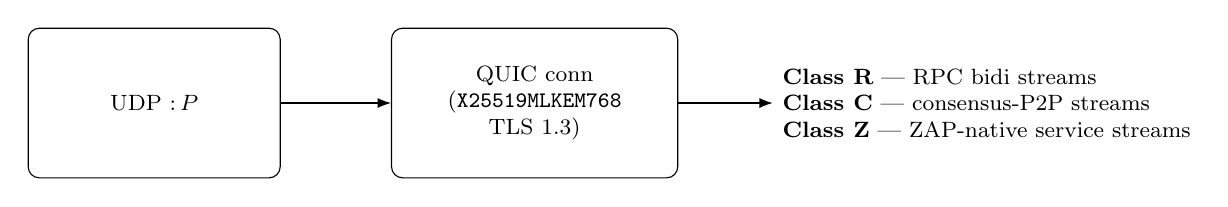
\begin{tikzpicture}[font=\footnotesize,node distance=4mm]
  \node[draw,rounded corners,align=center,minimum width=3.2cm,minimum height=1.9cm] (udp) {UDP :\,$P$};
  \node[draw,rounded corners,align=center,text width=3.4cm,right=1.4cm of udp,minimum height=1.9cm] (quic) {QUIC conn\\(\code{X25519MLKEM768}\\ TLS 1.3)};
  \node[right=1.2cm of quic,align=left] (streams)
    {\textbf{Class R} --- RPC bidi streams\\
     \textbf{Class C} --- consensus-P2P streams\\
     \textbf{Class Z} --- ZAP-native service streams};
  \draw[-{Latex}] (udp) -- (quic);
  \draw[-{Latex}] (quic) -- (streams);
\end{tikzpicture}
\end{center}

\subsection{Stream classes and demultiplexing}\label{sec:demux}

QUIC gives independent, individually reliable+ordered streams. We assign:

\begin{description}[nosep,leftmargin=1.6cm]
  \item[Class~R (RPC)] The \code{/ext/*} client API. \emph{One
        bidirectional stream per Call}: write one request frame, read one
        response frame, close. Replaces both \code{:9630} HTTP and
        \code{:9632} ZAP-RPC. Idempotent read RPCs MAY use 0-RTT; all
        others set \code{RejectEarlyData} (\S\ref{sec:0rtt}).
  \item[Class~C (consensus-P2P)] The Lux/Simplex message set
        (\S\ref{sec:consensus}). Request/response consensus exchanges
        (\msg{Get}/\msg{Put}, \msg{GetAncestors}/\msg{Ancestors},
        \msg{PushQuery}/\msg{PullQuery}$\to$\msg{Chits}) map to
        bidirectional streams; pure gossip
        (\msg{Ping}, \msg{Pong}, \msg{PeerList}, \msg{AppGossip},
        Simplex \msg{Vote}/\msg{Notarization}) maps to unidirectional
        streams. \emph{Never} 0-RTT.
  \item[Class~Z (ZAP-native)] Native ZAP services (\code{rpcdb},
        \code{rpcvm}, DA, messaging, and the \code{node2} vote frames).
        Framed \code{[4-BE len][1 msg\_type][payload]} with
        \code{msg\_type} demultiplexing to the service handler exactly as
        in \code{zap-cpp-core}.
\end{description}

\paragraph{Demux mechanism.} We do \emph{not} overload the reserved
flag bits of the ZAP \code{msg\_type} byte (\code{0x80}/\code{0x40}) for
class selection --- those keep their response/error meaning. Instead the
stream class is determined structurally and cheaply:

\begin{enumerate}[nosep]
  \item \textbf{Directionality.} Unidirectional streams are always gossip
        (Class~C uni or Class~Z one-way); bidirectional streams are
        request/response (Class~R or Class~C req/resp or Class~Z Call).
  \item \textbf{A 1-byte stream-class prefix} is written as the first
        byte of the first frame on every stream:
        \code{0x52 'R'}, \code{0x43 'C'}, \code{0x5A 'Z'}. The reader
        peeks one byte, routes the stream to the class dispatcher, and
        the remainder of the stream is that class's native framing. This
        keeps the three message schemas fully independent (orthogonal):
        Class~C stays byte-identical to the Lux message encoding,
        Class~Z stays byte-identical to \code{zap-cpp-core}, and neither
        needs to know the other exists.
\end{enumerate}

The class prefix is the \emph{only} new byte on the wire, and it lives
below all three payload schemas, so no existing message encoding changes.

\subsection{No head-of-line blocking}\label{sec:nohol}

On the TCP staking stream, a lost segment stalls \emph{all} subsequent
bytes until retransmission, and a large in-flight \msg{Ancestors}
transfer delays every message queued behind it. QUIC loss recovery and
flow control are \emph{per stream}: a lost packet on the bootstrap
stream does not delay a \msg{PushQuery} on another stream, and a
\SI{10}{\mega\byte} \msg{Ancestors} response cannot starve a
\SI{200}{\byte} \msg{Chits}. This strictly improves consensus message
latency under load and, as \S\ref{sec:bft} argues, can only help
liveness. It is the same property \code{node2}'s \code{FrameReader}
engineers by hand for its single-threaded pump --- here it is a
transport guarantee.

\subsection{0-RTT, migration, and their hazards}\label{sec:0rtt}

\paragraph{0-RTT (early data).} QUIC resumption lets a returning client
send application data in the first flight, saving a round trip. Early
data is \emph{replayable} by an active adversary
(\cite{rfc9001}~\S9.2). Policy:

\begin{itemize}[nosep]
  \item Class~R: permitted only for provably idempotent read RPCs; the
        server sets \code{RejectEarlyData} for every mutating handler.
  \item Class~C: \textbf{forbidden.} Consensus messages are never carried
        as 0-RTT early data. A replayed \msg{PushQuery} or \msg{Vote}
        must never be actionable off the resumption path; consensus
        streams open only after the handshake confirms (1-RTT).
  \item Class~Z: per-service, defaulting to forbidden.
\end{itemize}

This preserves the BFT model's assumption that a message is delivered
because a peer \emph{sent} it, not because an adversary \emph{replayed}
it (see G4 and \S\ref{sec:bft}).

\paragraph{Connection migration.} QUIC identifies a connection by
Connection ID, not by 4-tuple, so a validator surviving a NAT rebind or
an interface change (mobile/local-fiber uplink flap) keeps its
consensus connections alive across the address change. Migration is
authenticated by QUIC path validation; the peer identity
(\S\ref{sec:handshake}) is bound at handshake and does not re-open on
migration. \code{RemoteAddr} is therefore informational, not
authoritative --- the ML-DSA-bound \code{NodeID} is the identity, never
the IP.

\subsection{UDP at the edge}\label{sec:edge}

QUIC is UDP. Two deployment shapes:

\begin{itemize}[nosep]
  \item \textbf{Direct public IP} (recommended for validators): the UDP
        port is reachable directly; no L7 proxy sits in the consensus
        path. This is the natural fit for \S\ref{sec:dns}'s
        one-name-per-validator scheme.
  \item \textbf{L4 UDP load balancer} (e.g.\ DO LB in UDP mode): must
        forward UDP with source-address preservation or client-IP
        affinity; an L7/HTTP LB \emph{cannot} carry QUIC consensus
        traffic and must not be placed in the path. This is an explicit
        ops constraint, not a nice-to-have: QUIC path validation and
        migration require the LB to be transparent at L4.
\end{itemize}

Because RPC now shares the QUIC port, the public RPC edge also moves to
UDP/QUIC (HTTP/3). A classical HTTPS/H2 edge MAY be kept temporarily as a
translation layer for non-QUIC clients (\S\ref{sec:fallback}), but
validator-to-validator traffic is pure QUIC-PQ.

%======================================================================
\section{Post-quantum handshake and hybrid identity}\label{sec:handshake}

\subsection{Two layers, bound together}

The handshake has a \emph{key-agreement} layer and an
\emph{authentication} layer, and the novelty is the binding between
them.

\begin{description}[leftmargin=0pt]
  \item[Layer 1 --- Confidential channel (live).] The QUIC TLS~1.3
        handshake negotiates \code{X25519MLKEM768} (0x11EC). The session
        secret is IND-CCA if either X25519 or ML-KEM-768 holds
        (\cite{xwing,ghp2018combiners,bindel2019hybrid}); QUIC keys are
        forward-secret (ephemeral KEM shares). This satisfies G1. We
        deliberately use the \emph{IANA} hybrid group, not a Lux-private
        variant, so every TLS~1.3 stack in the estate speaks the same
        group.\footnote{Terminology: colloquially ``X-Wing.'' Precisely,
        the TLS group \code{X25519MLKEM768} uses the TLS-hybrid
        concatenation KDF, which is closely related to but not identical
        to the single-KEM X-Wing construction of ePrint 2024/039
        \cite{xwing}. Both are secure hybrid KEMs; we cite the analysis
        for the combiner family \cite{ghp2018combiners}.}
  \item[Layer 2 --- Hybrid identity (design).] Over the first
        bidirectional stream (the \emph{identity stream}, class-tag
        \code{'C'}, stream id 0), each side runs the ZAP-PQ \msg{AUTH}
        exchange (\S\ref{sec:proven-zappq}) \emph{channel-bound} to the
        QUIC session. This replaces the unauthenticated 64-byte
        \code{NodeID} string (\S\ref{sec:gap}).
\end{description}

\subsection{Channel binding}\label{sec:cb}

Let the completed QUIC/TLS session expose an RFC~5705 exporter
\cite{rfc5705}. Define the channel-binding value
\[
  \tau \;=\; \mathrm{TLS\text{-}Exporter}\bigl(\text{label}=\code{"lux-zap-pq-v1 channel-binding"},\ \text{context}=\text{chainID},\ 32\bigr).
\]
$\tau$ is a 32-byte value that is (i)~unique to this connection (depends
on the hybrid KEM transcript), (ii)~unknown to any party that did not
complete \emph{this} handshake, and (iii)~scoped to \code{chainID}. The
identity-stream \msg{AUTH} message is the SPEC-ZAP-PQ-v1 signature over
the transcript $H_2$ with $\tau$ folded in:
\[
  \mathsf{sig} \;=\; \mathrm{ML\text{-}DSA\text{-}65.Sign}_{\,sk}\Bigl(
     \mathsf{lbl}_{\text{proto}} \Vert \text{suite} \Vert H_2 \Vert \tau \Vert \mathsf{lbl}_{\text{role}}
  \Bigr),\quad \text{context}=\code{"lux-zap-pq-v1"}.
\]
Because $\tau$ binds the signature to \emph{this} QUIC session and to
\code{chainID}, an \msg{AUTH} captured on one connection is worthless on
another (G4): a MITM who terminates TLS with its own certificate obtains
a \emph{different} $\tau$ and cannot reuse the victim's ML-DSA signature;
a cross-chain replay sees a different context. This is the QUIC analogue
of luxd's existing chain-ID-bound \code{PQHandshake}
(\S\ref{sec:proven-pqid}); we reuse that design rather than invent one.

\subsection{The hybrid \texttt{NodeID}}\label{sec:nodeid}

We preserve the classical value and pair it with the PQ value.

\begin{definition}[Hybrid validator identity]\label{def:hybrid}
A validator's identity is the pair
$\bigl(\code{NodeID}_{\mathrm{cls}},\ pk_{\mathrm{pq}}\bigr)$ where
\[
  \code{NodeID}_{\mathrm{cls}} = \mathrm{RIPEMD160}\bigl(\mathrm{SHA256}(\text{cert}.\mathrm{Raw})\bigr),
  \qquad
  pk_{\mathrm{pq}} = \text{ML-DSA-65 public key},
\]
cross-bound by two signatures published at registration: the staking
key signs $pk_{\mathrm{pq}}$ and $pk_{\mathrm{pq}}$ signs
$\code{NodeID}_{\mathrm{cls}}$, each under a domain-separated context.
The active \code{NodeID} under a PQ profile is
$\code{NodeID}_{\mathrm{pq}} = \code{NodeIDSchemeMLDSA65.DeriveMLDSA}(\text{chainID}, pk_{\mathrm{pq}})$,
the scheme luxd already ships (\S\ref{sec:proven-pqid}).
\end{definition}

\begin{claim}[Identity continuity, G3]
Under \code{ProfilePermissive}, the validator-set key remains
$\code{NodeID}_{\mathrm{cls}}$ (20 bytes), so no stake-map migration is
forced; the ML-DSA leg is additive authentication. Under
\code{ProfileStrictPQ}, the key is $\code{NodeID}_{\mathrm{pq}}$, and the
cross-binding lets verifiers that still track $\code{NodeID}_{\mathrm{cls}}$
follow the transition without a flag day.
\end{claim}

\begin{claim}[Hybrid unforgeability, G2]
To present as validator $V$ on a QUIC-PQ connection an adversary must
produce a valid channel-bound ML-DSA-65 signature under $V$'s
$pk_{\mathrm{pq}}$ \emph{and} complete a TLS handshake with $V$'s staking
certificate. Under EUF-CMA of ML-DSA-65 (FIPS-204 \cite{fips204}) the
first is infeasible without $sk_{\mathrm{pq}}$; a quantum forger who
breaks only the classical staking key still cannot forge the ML-DSA
leg. Conversely a lattice adversary who forges ML-DSA but not the
classical credential fails the TLS leg under \code{ProfilePermissive}.
Impersonation requires breaking \emph{both} --- the X-Wing pattern for
identity.
\end{claim}

\subsection{Handshake flow (design)}\label{sec:flow}

\begin{enumerate}[nosep]
  \item QUIC/TLS 1.3 handshake; negotiate \code{X25519MLKEM768}, ALPN
        \code{"zap/1"}. [live]
  \item Both sides derive $\tau$ from the TLS exporter (\S\ref{sec:cb}).
  \item Client opens the identity stream (bidi, class \code{'C'},
        id~0), sends
        $\langle pk_{\mathrm{pq}},\ \mathsf{sig}_I,\ \code{NodeID}_{\mathrm{cls}},\ \text{cross-bind sigs}\rangle$.
  \item Server verifies $\mathsf{sig}_I$ over $(H_2,\tau,\text{role}=I)$,
        checks $pk_{\mathrm{pq}}\!\to\!\code{NodeID}$ under the active
        scheme, checks validator-set membership, then replies with its
        own $\langle pk_{\mathrm{pq}},\ \mathsf{sig}_R,\ \dots\rangle$.
  \item Client verifies symmetrically. On success both sides hold a
        mutually-authenticated, PQ-confidential, channel-bound
        connection whose \code{NodeID} is trustworthy. Consensus streams
        (Class~C, 1-RTT only) may now open.
\end{enumerate}

Reuse map: step~1 is \code{luxfi/zap/quic} verbatim; the \msg{AUTH}
signature/verify in steps 3--5 is
\code{zap/handshake.Identity.Sign}/\code{VerifyAuth} with $\tau$ added to
the sign-input; the \code{NodeID} derivation is luxd's
\code{NodeIDSchemeMLDSA65}. No new cryptographic code, only the binding
of $\tau$ and the stream plumbing.

%======================================================================
\section{Consensus-P2P over QUIC-ZAP}\label{sec:consensus}

\subsection{The message set is unchanged}

The Lux/Simplex message set (\code{proto/p2p}) is carried
byte-for-byte. We change \emph{where the bytes travel}, not the bytes.
Table~\ref{tab:msgmap} gives the stream map.

\begin{table}[h]\centering\small
\begin{tabular}{@{}lll@{}}
\toprule
\textbf{Category} & \textbf{Messages} & \textbf{QUIC stream} \\
\midrule
Handshake/net & \msg{Handshake}, \msg{GetPeerList}, \msg{PeerList}, \msg{Ping}, \msg{Pong} & uni (gossip); identity on bidi id 0 \\
State-sync & \msg{GetStateSummaryFrontier}, \msg{StateSummaryFrontier}, & bidi req/resp \\
           & \msg{GetAcceptedStateSummary}, \msg{AcceptedStateSummary} & \\
Bootstrap & \msg{GetAcceptedFrontier}, \msg{AcceptedFrontier}, \msg{GetAccepted}, & bidi req/resp \\
          & \msg{Accepted}, \msg{GetAncestors}, \msg{Ancestors} & (own stream: large, HOL-isolated) \\
Consensus & \msg{Get}, \msg{Put}, \msg{PushQuery}, \msg{PullQuery}, \msg{Chits} & bidi req/resp, 1-RTT \\
App & \msg{AppRequest}, \msg{AppResponse}, \msg{AppGossip}, \msg{AppError} & bidi (req/resp) / uni (gossip) \\
Simplex & \msg{BlockProposal}, \msg{Vote}, \msg{EmptyVote}, \msg{Notarization} & uni (gossip), 1-RTT \\
\bottomrule
\end{tabular}
\caption{Lux/Simplex messages to QUIC stream classes. Semantics
are preserved: a request expects one response; gossip expects none.
Large bootstrap transfers get their own streams so they cannot
HOL-block votes (\S\ref{sec:nohol}).}
\label{tab:msgmap}
\end{table}

\subsection{Drop-in compatibility via the \texttt{net.Conn} seam}\label{sec:seam}

luxd's peer layer is already transport-abstract. Inbound goes through
\[
  \code{Upgrader.Upgrade}(\code{net.Conn}) \to (\code{NodeID},\ \code{net.Conn},\ \text{*Certificate},\ \text{err}),
\]
and outbound through \code{EndpointDialer} (which already carries TCP,
DNS, and an RNS mesh transport). Two integration levels:

\begin{description}[nosep,leftmargin=1.2cm]
  \item[L0 --- Conservative drop-in.] A QUIC \code{Upgrader} completes
        the handshake of \S\ref{sec:flow} and returns a \code{net.Conn}
        that \emph{is} one bidirectional QUIC stream. The existing
        message read/write loop runs over it unchanged; message framing
        is byte-identical to TCP. This yields PQ security and the
        single-port collapse with \emph{zero} change to the consensus
        message loop --- the minimal, safest first step, and the one the
        A/B test (\S\ref{sec:ab}) should gate on.
  \item[L1 --- Full multiplex.] The peer layer is taught to open a
        stream per message class (Table~\ref{tab:msgmap}), unlocking the
        no-HOL win (\S\ref{sec:nohol}) and per-Call RPC parallelism. This
        is a peer-layer change \emph{above} the transport and \emph{below}
        BFT; it does not alter message semantics. It is opt-in and can
        ship after L0 is proven.
\end{description}

Crucially the \code{Upgrader} contract already returns the
$(\code{NodeID}, \code{net.Conn}, \text{cert})$ triple the network
expects, so the consensus layer (\code{network.NewNetwork}) is oblivious
to which transport produced the conn. This is the decomplection that
makes the change safe.

\subsection{Reusing the \texttt{node2} vote-mesh}\label{sec:votemesh}

The Simplex \msg{Vote}/\msg{Notarization} path is precisely what
\code{node2} already runs: a \code{SignedVote}
(\code{block\_id\,$\Vert$\,voter\,$\Vert$\,sig}) gossiped as a ZAP frame,
verified and de-duplicated by the gate, finalised by a $>2/3$-stake
quorum certificate. Over QUIC-ZAP the same \code{encode\_vote} /
\code{decode\_vote} codec (with its strict no-trailing-bytes
non-malleability check) is written to a Class~C unidirectional stream
instead of a raw socket, and \code{FrameReader}'s hand-rolled non-blocking
reassembly is subsumed by QUIC's per-stream delivery. The proven wire
semantics (\S\ref{sec:proven-node2}) are unchanged; only the byte
carrier changes. This is the C++ vote-mesh and the Go peer layer meeting
at the same ZAP frame.

%======================================================================
\section{Fallback negotiation and mixed fleets}\label{sec:fallback}

\subsection{Baseline and capability}

The proven classical TCP staking listener on \code{9631/tcp} is the
permanent baseline. A validator additionally binds \code{9631/udp} for
QUIC-PQ. QUIC-PQ is a \emph{capability} discovered three ways
(any one suffices):

\begin{enumerate}[nosep]
  \item \textbf{Handshake capability bit.} The \msg{Handshake}/\msg{Version}
        message gains an optional \code{transports} field advertising
        \code{quic-pq/1}. Absent the field, the peer is TCP-only. (A new
        \emph{optional} field is backwards-compatible with the proto.)
  \item \textbf{DNS advertisement.} A \code{SRV}/\code{TXT} record
        (\S\ref{sec:dns}) publishes the UDP port and \code{quic-pq/1}.
  \item \textbf{mDNS} on local segments (\code{luxfi/zap} already ships
        mDNS discovery), for datacenter/local-fiber clusters.
\end{enumerate}

\subsection{Upgrade rule}

\begin{center}\small
\begin{tabular}{@{}lll@{}}
\toprule
\textbf{Peer A} & \textbf{Peer B} & \textbf{Result} \\
\midrule
QUIC-PQ & QUIC-PQ & QUIC-PQ (both advertise; dial UDP; TCP idle) \\
QUIC-PQ & TCP-only & TCP \code{9631} (proven path) \\
TCP-only & QUIC-PQ & TCP \code{9631} \\
TCP-only & TCP-only & TCP \code{9631} \\
\bottomrule
\end{tabular}
\end{center}

The rule is monotone: presence of the capability on \emph{both} sides is
necessary and sufficient to use QUIC-PQ; otherwise the fleet
transparently uses the classical path. A validator runs both listeners
concurrently, so the fleet is a free mix of upgraded and legacy nodes
with no partition (G6). Anti-downgrade: once both peers have advertised
\code{quic-pq/1} (a value carried \emph{inside} the authenticated
\msg{Handshake} on whichever transport bootstrapped them), a silent
downgrade to TCP by a network adversary is detectable --- the peers
expected QUIC and can log/refuse per policy. Because both transports
deliver the \emph{same} authenticated message stream to the same BFT
logic, correctness never depends on which was chosen; the anti-downgrade
check is a monitoring and policy affordance, not a safety dependency.

\subsection{Migration discipline}

TCP \code{9631} is retired for a network \emph{only} after the A/B gate
(\S\ref{sec:ab}) shows byte-identical finality on that network for a
sustained window. Order: devnet $\to$ testnet $\to$ mainnet, each
gated independently. This mirrors the estate's standing rollout
discipline (canary, then atomic $\ge$ quorum).

%======================================================================
\section{DNS scheme and validator onboarding}\label{sec:dns}

\subsection{One name per validator per network}

\begin{center}\small
\begin{tabular}{@{}lll@{}}
\toprule
\textbf{Network} & \textbf{Zone} & \textbf{Validator name} \\
\midrule
mainnet & \code{lux.network} & \code{$\langle$NN$\rangle$.lux.network} \\
testnet & \code{lux-test.network} & \code{$\langle$NN$\rangle$.lux-test.network} \\
devnet  & \code{lux-dev.network} & \code{$\langle$NN$\rangle$.lux-dev.network} \\
\bottomrule
\end{tabular}
\end{center}

\code{NN} is a zero-padded index (\code{01}, \code{02}, \dots); local
fiber DEX validators occupy \code{06} and up. Each name resolves to:

\begin{itemize}[nosep]
  \item \code{A}/\code{AAAA} --- the validator's public IP;
  \item \code{SRV} \code{\_zap-quic.\_udp.$\langle$NN$\rangle$.$\langle$zone$\rangle$}
        --- the QUIC-PQ UDP port and priority/weight;
  \item \code{TXT} --- capability string \code{quic-pq/1}, and the
        \emph{fingerprint} of the validator's $pk_{\mathrm{pq}}$
        (SHA3-256), so a resolver can pin the expected ML-DSA identity
        before dialing (DNS is advisory; the handshake is authoritative).
\end{itemize}

DNS is a \emph{discovery} convenience only. Peer identity is never DNS
--- it is the channel-bound ML-DSA \code{NodeID} of \S\ref{sec:handshake}.
A poisoned DNS answer can at worst deny service (wrong IP) or trigger a
handshake that fails identity verification; it cannot cause acceptance of
a wrong validator.

\subsection{Local-fiber / NAT validator join}\label{sec:join}

A validator behind a home/office fiber uplink (the \code{06+} local DEX
validators) joins as follows:

\begin{enumerate}[nosep]
  \item \textbf{Key + identity.} Generate the staking cert and the
        ML-DSA-65 keypair; compute
        $(\code{NodeID}_{\mathrm{cls}}, pk_{\mathrm{pq}})$ and the
        cross-binding signatures (Def.~\ref{def:hybrid}).
  \item \textbf{Register on P-chain.} \code{AddPermissionlessValidator}
        with the hybrid identity (the P-chain tx carries the staking key;
        $pk_{\mathrm{pq}}$ is bound per \S\ref{sec:proven-pqid}). This is
        unchanged from today except that the PQ key is included.
  \item \textbf{Publish endpoint.} Set \code{A}/\code{SRV}/\code{TXT} for
        \code{$\langle$NN$\rangle$.lux-dev.network} (or the operator's own
        name; the \code{NN} scheme is a convention, and \code{TXT}
        capability discovery works under any name).
  \item \textbf{Reachability.} QUIC is UDP, so a single inbound UDP port
        forward on the CPE suffices; QUIC connection migration
        (\S\ref{sec:0rtt}) tolerates the periodic public-IP change of a
        residential uplink without dropping consensus connections. Where
        no inbound port is possible, the validator dials out to
        already-reachable peers and QUIC keeps the bidirectional
        connection open (consensus is symmetric over an established
        conn); NAT hole-punching via a rendezvous peer is a future option
        but not required for the common single-port-forward case.
  \item \textbf{Peer over QUIC-PQ.} Discover peers via DNS/mDNS, dial
        their \code{SRV} UDP endpoints, complete the \S\ref{sec:flow}
        handshake, and begin exchanging the (unchanged) consensus
        messages.
\end{enumerate}

%======================================================================
\section{Devnet A/B acceptance: byte-identical finality}\label{sec:ab}

The retirement gate for the fallback is an empirical equality, not an
argument. Run the \emph{same} validator set finalising the \emph{same}
chain twice:

\begin{description}[nosep,leftmargin=1.4cm]
  \item[Run A] all consensus-P2P over TCP \code{9631} (baseline).
  \item[Run B] all consensus-P2P over QUIC-PQ (\S\ref{sec:consensus}, at
        integration level L0 first, then L1).
\end{description}

\begin{definition}[Acceptance]\label{def:accept}
Runs A and B \emph{pass} iff, for every height $h$ in the test window,
they agree on: the accepted block id and full block bytes at $h$; the
accepted frontier; and the finality certificate bytes (the BLS/Simplex
quorum certificate, including the vote set and aggregate signature). Any
divergence is a fail.
\end{definition}

Because the transport is strictly below the message layer and the
message bytes are identical between A and B, finality \emph{must} be
identical; the test \emph{proves} the transport introduced no semantic
change (any difference indicts the transport). The C++ analogue is
already green: \code{node2}'s \code{cluster\_5} finalises with a
verifying $>2/3$-stake certificate over the ZAP mesh
(\S\ref{sec:proven-node2}); the Go devnet A/B lifts that guarantee to
the full luxd message set.

\paragraph{Instrumentation.} Compare via the finality ledger's
per-height certificate bytes and \code{LastAccepted} at matched heights;
diff block bytes by hash. Run each arm $\ge 3$ times to rule out
nondeterministic scheduling; require bitwise equality of the certificate
set (order-normalised by validator index, as the certificate encoding
already prescribes).

%======================================================================
\section{BFT preservation argument}\label{sec:bft}

\begin{assumption}[Message-layer BFT, unchanged]\label{as:bft}
Under partial synchrony \cite{dwork1988consensus} with $<n/3$ Byzantine
stake and an \emph{authenticated} network that eventually delivers
messages between honest parties within $\Delta$ after GST, the
Lux/Simplex protocol is safe (no two honest nodes finalise
conflicting blocks at a height) and live (honest transactions eventually
finalise). This is proven at the message layer (LP-020
\cite{lp020quasar}) and is \emph{not} re-proven here.
\end{assumption}

\begin{theorem}[Transport transparency]\label{thm:transparent}
Replacing the TCP staking transport with QUIC-PQ (\S\ref{sec:consensus},
integration L0 or L1) preserves the safety and liveness of
Assumption~\ref{as:bft}.
\end{theorem}

\begin{proof}[Proof sketch]
The BFT protocol consumes a stream of \emph{authenticated messages} and
requires two properties of the transport: (P1)~\emph{authentication} ---
a message attributed to honest $V$ was sent by $V$; (P2)~\emph{eventual
delivery} --- after GST, a message between honest parties arrives within
$\Delta$. We show QUIC-PQ provides both at least as strongly as
TCP-TLS.

\emph{Safety.} Safety depends only on (P1) and on the message contents,
not on ordering across distinct messages (each \msg{Vote}/\msg{Chits} is
independently attributable and idempotently counted; the gate
de-duplicates by voter key, exactly as \code{node2} does). QUIC-PQ
strengthens (P1): every message rides a connection whose \code{NodeID} is
bound by a channel-bound ML-DSA-65 signature (\S\ref{sec:cb}), which is
$\ge$ the TLS-cert binding of the classical path and additionally
PQ-secure. The consensus message bytes are identical (\S\ref{sec:consensus}),
so the set of finalisable decisions is unchanged. The one transport-level
way to \emph{violate} (P1) would be actionable replay; we forbid 0-RTT
on Class~C (\S\ref{sec:0rtt}), so no consensus message is delivered
except as authenticated 1-RTT data. Hence no new equivocation or
double-count is possible, and safety is preserved.

\emph{Liveness.} QUIC provides per-stream reliable, ordered delivery ---
the same guarantee TCP gives per connection --- so after GST honest
messages are delivered within a $\Delta$ no larger than TCP's (QUIC's
loss recovery is comparable to TCP's, and its handshake is $\le$ one
extra flight, amortised by 0-RTT for idempotent RPC). Moreover per-stream
independence \emph{removes} cross-message HOL blocking (\S\ref{sec:nohol}):
a stalled bootstrap transfer no longer delays a consensus vote, which can
only \emph{decrease} effective message latency under load. Connection
migration (\S\ref{sec:0rtt}) preserves liveness across address changes
that would drop a TCP connection and force re-dial. Thus (P2) holds with
a $\Delta$ no worse --- typically better --- than the baseline, and
liveness is preserved.

Since both required properties are met, Assumption~\ref{as:bft}'s
conclusions carry over unchanged. $\square$
\end{proof}

\begin{claim}[The $f<n/3$ bound is untouched]
The fault threshold is a property of the \emph{decision rule} and the
\emph{validator set}, both unchanged. The transport neither adds nor
removes validators, neither weakens nor strengthens the quorum
arithmetic; it only carries the same votes among the same set. The
A/B test (\S\ref{sec:ab}) is the empirical confirmation of
Theorem~\ref{thm:transparent}.
\end{claim}

%======================================================================
\section{Minimal proof-of-concept}\label{sec:poc}

Two cheap, self-contained artifacts de-risk the design without touching
consensus:

\begin{enumerate}[nosep]
  \item \textbf{QUIC-PQ echo + CurveID assertion.} A client/server that
        opens a \code{luxfi/zap/quic} connection, asserts
        \code{ConnectionState().CurveID == 0x11EC}, opens the three
        stream classes (R/C/Z), writes a class-prefixed frame on each,
        and echoes it back --- proving the demux (\S\ref{sec:demux}) and
        that PQ key agreement is really negotiated. (The CurveID
        assertion already exists in \code{quic}'s test suite; the PoC adds
        the three-class prefix and round-trips one frame per class.)
  \item \textbf{Channel-bound AUTH over a QUIC stream.} On stream id~0,
        run \code{zap/handshake.Identity.Sign}/\code{VerifyAuth} with the
        RFC-5705 exporter $\tau$ folded into the sign-input
        (\S\ref{sec:cb}); assert that a signature produced against one
        connection's $\tau$ fails verification against another
        connection --- the channel-binding property (G4), demonstrated as
        a negative test.
\end{enumerate}

Both live in \code{luxfi/zap} (transport + handshake) and require no
change to luxd's consensus or proposer VM, matching the scope guardrail.
They are the executable core of \S\ref{sec:wire}--\S\ref{sec:handshake};
the luxd \code{Upgrader}/\code{EndpointDialer} wiring (\S\ref{sec:seam})
and the A/B harness (\S\ref{sec:ab}) are the follow-on integration.

%======================================================================
\section{Related Lux work}\label{sec:related}

This paper is the transport capstone of the ZAP stack. LP-200
\cite{lp200zapstack} is the ten-layer umbrella; LP-201
\cite{lp201universalwire} is the universal wire format whose frames ride
these streams; LP-9702 \cite{lp9702zwing} is the Z-Wing hybrid PQ secure
channel we reuse as the identity layer; LP-020 \cite{lp020quasar} is the
consensus whose messages this transport carries unchanged. The
\code{node2}/\code{consensus2} vote-mesh is the C++ realisation of the
Class~C gossip path. Against upstream Avalanche, the sole delta is the
transport and the hybrid identity binding; the message set and BFT logic
are preserved verbatim (the ``extend, don't break'' guardrail).

%======================================================================
\section{Conclusion}\label{sec:conclusion}

One UDP port per validator, QUIC over ZAP, end-to-end post-quantum: RPC,
consensus-P2P, and ZAP-native services multiplexed as independent QUIC
streams over an \code{X25519MLKEM768} channel with a channel-bound
ML-DSA-65 hybrid \code{NodeID}. The design is composition over invention
--- every primitive is already proven and live; the new work is a channel
binding, a three-class demux, and the luxd transport-seam wiring. The
classical TCP path remains the negotiated fallback until a
devnet A/B test proves byte-identical finality, and a message-layer
argument shows the transport swap cannot alter $f<n/3$ safety or
liveness. The result collapses three endpoints and three security
postures into one, removes transport head-of-line blocking from the
consensus path, and makes every validator connection quantum-safe by
default --- without touching a line of the BFT decision logic.

\bibliographystyle{plain}
\bibliography{biblio}

\end{document}
